\documentclass{article}

\usepackage[preprint]{neurips_2026}

\usepackage[utf8]{inputenc}
\usepackage[T1]{fontenc}
\usepackage{hyperref}
\usepackage{url}
\usepackage{booktabs}
\usepackage{amsfonts}
\usepackage{amsmath}
\usepackage{nicefrac}
\usepackage{microtype}
\usepackage{graphicx}
\usepackage{xcolor}
\usepackage{subcaption}
\usepackage{multirow}

\graphicspath{{figures/}}

\title{Cross-Generational Transfer of Adversarial Attacks Reveals \\
Non-Monotonic Safety Alignment in LLMs}

\author{%
  Subhadip Mitra\thanks{This paper builds on the quality-diversity adversarial framework introduced in our prior work~\citep{mitra2026qd}, which appeared at the ICLR 2026 Workshop on Agents in the Wild (AIWILD).}\\
  Research Lead, Rota Labs\\
  \texttt{subhadip@rotalabs.ai}\\
}

\begin{document}

\maketitle

\begin{abstract}
Safety alignment in LLMs does not improve monotonically across model
generations. Studying four generations of Google's Gemma family
(7B--31B) with quality-diversity evolution (MAP-Elites) as an automated
red-teaming probe, we find that Gemma~3 (12B) exhibits
$68.7\% \pm 5.7\%$ attack success rate (ASR; mean $\pm$ std, 3 seeds),
significantly higher than its predecessor Gemma~2
($45.5\% \pm 7.2\%$; $p = 0.030$, paired bootstrap) and its successor
Gemma~4 ($33.9\% \pm 1.8\%$). Replaying evolved attack archives across
generations reveals that attacks from \emph{other} generations transfer
to Gemma~3 at 44--46\% but only 14--18\% to Gemma~4, indicating that
Gemma~4's safety gains generalize beyond the attack distributions
evolved against earlier generations. Under our 8B judge, copyright and
cybercrime vulnerabilities register at near-100\% across all
generations, though a second-judge audit (\S\ref{sec:discussion})
suggests the copyright result is sensitive to judge choice.
Misinformation ASR jumps from 29\% to 99\% between Gemma~2 and
Gemma~3 and remains elevated at 77\% in Gemma~4, indicating the
regression was not fully addressed. These patterns are invisible to
static benchmarks and emerge only through adaptive, longitudinal
probing. All experiments use 3 random seeds with a unified self-hosted
judge; code and artifacts are available at
\url{https://github.com/bassrehab/red-queen}.
\end{abstract}

%% ============================================================================
\section{Introduction}
\label{sec:intro}

Large language model (LLM) safety alignment has improved rapidly, but
measuring that improvement rigorously remains an open challenge.
Static benchmarks such as HarmBench~\cite{mazeika2024harmbench} and
AdvBench~\cite{zou2023universal} provide point-in-time snapshots but
do not capture how an adaptive adversary interacts with evolving defenses.

A fundamental question is whether safety improvements \emph{generalize}:
when a model developer patches vulnerabilities between releases, do old
attacks stop working (indicating targeted fixes), or does the model become
broadly more robust? Answering this requires a methodology for
\emph{differential safety probing}: systematically comparing safety
surfaces across model versions with a consistent adversarial process.

In this paper, we address two specific questions:
\begin{enumerate}
    \item \textbf{Cross-generational transfer:} Do adversarial attacks
          evolved against an earlier model generation transfer to later
          generations of the same family?
    \item \textbf{Non-monotonic robustness:} Does safety alignment
          improve consistently across model generations, or can it
          regress?
\end{enumerate}

We study these questions using four generations of Google's Gemma model
family (7B, 9B, 12B, 31B parameters), spanning releases from 2024 to 2026.
Our probe is a quality-diversity (QD) evolutionary algorithm (MAP-Elites)
that discovers diverse jailbreak strategies across seven harm categories
from the HarmBench taxonomy. By evolving attack archives against each model
with 3 independent seeds and replaying them across generations, we
construct a transfer matrix with uncertainty estimates that reveals which
vulnerabilities persist and which are patched.

\paragraph{Contributions.}
\begin{itemize}
    \item A QD-evolution methodology for \emph{differential safety probing}
          that enables systematic, reproducible comparison of safety surfaces
          across model versions (\S\ref{sec:method}).
    \item A cross-generational transfer analysis across four Gemma
          generations, revealing that attack transfer is generation-dependent
          and that Gemma~3 represents a statistically significant safety
          regression ($p = 0.030$; \S\ref{sec:results:transfer}).
    \item Empirical evidence that adversarial robustness does not improve
          monotonically across model generations within a single family,
          with a non-monotonic pattern coinciding with an architectural
          transition
          (\S\ref{sec:results:scaling}).
    \item Category-level analysis showing that some harm categories
          (notably copyright, under our 8B judge) appear to resist
          safety alignment across all generations while others show
          broadly declining trajectories
          (\S\ref{sec:discussion}).
\end{itemize}

%% ============================================================================
\section{Related Work}
\label{sec:related}

\paragraph{Automated red-teaming.}
Recent work has developed automated methods for discovering LLM
vulnerabilities, including gradient-based attacks
(GCG;~\cite{zou2023universal}), LLM-based attackers
(PAIR~\cite{chao2023jailbreaking}; TAP~\cite{mehrotra2024tree}),
and template-based approaches (AutoDAN~\cite{liu2024autodan}).
These methods target individual models; none study how discovered
vulnerabilities transfer across model generations.

\paragraph{Safety benchmarks.}
HarmBench~\cite{mazeika2024harmbench} provides a standardized taxonomy
of harmful behaviors across seven categories.
StrongREJECT~\cite{souly2024strongreject} proposes improved evaluation
metrics. We use HarmBench as our behavior taxonomy and seed pool,
enabling category-level transfer analysis.

\paragraph{Quality-diversity optimization.}
MAP-Elites~\cite{mouret2015illuminating} maintains a grid of diverse,
high-performing solutions across behavioral dimensions. Prior work has
applied QD methods to game playing~\cite{fontaine2020covariance} and
robot design~\cite{cully2015robots}.
In prior work~\citep{mitra2026qd}, we established that MAP-Elites
discovers more diverse LLM vulnerabilities than standard evolutionary
search, in a single-model setting. We adopt that probe and extend it in
three directions: a cross-generational transfer replay protocol,
a four-generation longitudinal study with three seeds per model,
and the empirical finding that safety alignment regresses
non-monotonically across Gemma generations.

\paragraph{Scaling laws.}
Scaling laws for LLM capabilities are well-established~\cite{kaplan2020scaling,
hoffmann2022training}. Whether safety properties follow similar predictable
scaling is largely unexplored. We provide evidence that adversarial
robustness does \emph{not} scale monotonically within a single model
family, a finding that contrasts with the regularity observed in
capability scaling.

%% ============================================================================
\section{Methodology}
\label{sec:method}

\subsection{Quality-Diversity Adversarial Probing}
\label{sec:method:qd}

We use MAP-Elites to evolve a diverse archive of jailbreak attacks against
a target LLM. Each attack is characterized by a genome encoding:
\begin{itemize}
    \item \textbf{Attack strategy} (6 types): roleplay, encoding,
          authority impersonation, hypothetical framing, multi-turn, and
          direct jailbreak.
    \item \textbf{Encoding} (6 types): none, Base64, ROT13, leetspeak,
          pig latin, Unicode substitution.
    \item \textbf{Seed behavior}: drawn from HarmBench's 400 behaviors
          across 7 semantic categories.
\end{itemize}

The MAP-Elites archive is a 3D grid indexed by
(strategy $\times$ encoding $\times$ harm category), with each cell
storing the highest-fitness attack for that behavioral niche. Fitness is
evaluated by a self-hosted LLM judge (Llama-3.1-8B-Instruct) that
classifies each target response along three binary axes: refusal,
harmful content, and relevance. The resulting score ranges from 0
(refused) to 1 (harmful and relevant). Using a single, self-hosted judge
for \emph{all} phases (evolution and transfer replay) ensures scoring
consistency and full reproducibility.

Each model is probed with 3 independent random seeds (42, 1337, 2718)
to estimate cross-seed variance. All evolution uses deterministic RNG
(ChaCha8, seeded) with ordered evaluation to ensure reproducibility
given the same seed.

\subsection{Cross-Generational Transfer Protocol}
\label{sec:method:transfer}

After evolving an archive $\mathcal{A}_{i,s}$ against model $M_i$ with
seed $s$, we \emph{replay} each archive against all other models
$M_j$ ($j \neq i$):
\begin{enumerate}
    \item For each entry in $\mathcal{A}_{i,s}$, send the attack prompt to
          $M_j$ and obtain the response.
    \item Score the response using the same LLM judge.
    \item Record per-entry and per-category transfer success.
\end{enumerate}

This produces a transfer tensor $T[i,j,s]$ where each entry is the
fraction of attacks from $\mathcal{A}_{i,s}$ that succeed against $M_j$.
We report the mean and standard deviation across seeds.
The diagonal $\bar{T}[i,i]$ is the mean self-evaluation success rate.
Off-diagonal entries reveal:
\begin{itemize}
    \item \textbf{Forward transfer} ($i < j$): old attacks on newer models.
          High values suggest safety improvements are superficial.
    \item \textbf{Backward transfer} ($i > j$): newer attacks on older
          models. High values suggest attacks exploit longstanding weaknesses.
\end{itemize}

\subsection{Robustness Across Generations}
\label{sec:method:scaling}

We plot robustness $R = 1 - \text{ASR}$ as a function of model
generation (with parameter count on the axis) to visualize the
trajectory of safety alignment within the Gemma family. We treat the
four generations as a case study and test specific pairwise
contrasts with paired bootstrap tests ($p < 0.05$, uncorrected;
$N = 3$ seeds limits power for multiple-testing correction).

%% ============================================================================
\section{Experimental Setup}
\label{sec:setup}

\subsection{Models}

\begin{table}[t]
\centering
\caption{Models evaluated. All served via vLLM~0.19.1 (bf16, temperature 0)
on a single NVIDIA H200 (141\,GB). Judge: self-hosted Llama-3.1-8B-Instruct
on NVIDIA RTX~4090 (24\,GB).}
\label{tab:models}
\begin{tabular}{llccc}
\toprule
\textbf{Model} & \textbf{Family} & \textbf{Params} & \textbf{Release} & \textbf{Architecture} \\
\midrule
Gemma 1 (7B-it)\textsuperscript{a}   & Gemma & 7B  & 2024 & Text-only \\
Gemma 2 (9B-it)\textsuperscript{b}   & Gemma & 9B  & 2024 & Text-only \\
Gemma 3 (12B-it)\textsuperscript{c}  & Gemma & 12B & 2025 & Multimodal \\
Gemma 4 (31B-it)\textsuperscript{d}  & Gemma & 31B & 2026 & Multimodal \\
\bottomrule
\end{tabular}
\\[2pt]
{\footnotesize
\textsuperscript{a}\texttt{google/gemma-7b-it}\quad
\textsuperscript{b}\texttt{google/gemma-2-9b-it}\quad
\textsuperscript{c}\texttt{google/gemma-3-12b-it}\quad
\textsuperscript{d}\texttt{google/gemma-4-31B-it}
}
\end{table}

We note that Gemma~3 and Gemma~4 introduced multimodal (vision-language)
capabilities, representing an architectural shift from the text-only
Gemma~1 and Gemma~2. This distinction is relevant to interpreting the
safety regression observed in Gemma~3 (\S\ref{sec:discussion}).

\subsection{Evolution Configuration}

MAP-Elites with $6 \times 6 \times 8$ grid (strategy $\times$ encoding
$\times$ category), yielding 288 behavioral niches. Batch size 50,
200 generations per model per seed, concurrency 5 parallel evaluations.
Mutation rate 0.3, crossover rate 0.7.
Seed pool: 400 HarmBench behaviors across 7 categories.
Three seeds per model (42, 1337, 2718) yield 12 evolution runs total.
Transfer replay: 36 source--target pairs (4 models $\times$ 3 other
targets $\times$ 3 seeds).

\subsection{Compute}

All Gemma models served sequentially on a single NVIDIA H200
(141\,GB HBM3e) via vLLM~0.19.1. LLM judge (Llama-3.1-8B-Instruct)
served on a dedicated NVIDIA RTX~4090 (24\,GB).
Total GPU time: approximately 60 hours across both machines
(12 evolution runs at $\sim$4 hours each, 36 transfer replays at
$\sim$8 minutes each, plus 4 raw-seed baselines and a 70B judge audit).

%% ============================================================================
\section{Results}
\label{sec:results}

\subsection{Baseline Attack Success Rates}
\label{sec:results:baseline}

Table~\ref{tab:asr} presents attack success rates (ASR) across all
HarmBench categories for each Gemma generation, reported as mean $\pm$
standard deviation across 3 seeds. The most striking observation is
the \emph{non-monotonic} pattern: overall ASR decreases from
$59.4\% \pm 3.0\%$ (Gemma~1) to $45.5\% \pm 7.2\%$ (Gemma~2), then
\emph{increases} to $68.7\% \pm 5.7\%$ (Gemma~3), before dropping to
its lowest value of $33.9\% \pm 1.8\%$ (Gemma~4).

The improvement from Gemma~1 to Gemma~2 ($p = 0.032$) and the
regression from Gemma~2 to Gemma~3 ($p = 0.030$) are both statistically
significant under paired bootstrap tests. The recovery from Gemma~3 to
Gemma~4, while large in absolute terms ($-34.8$ percentage points),
does not reach significance at $p < 0.05$ with 3 seeds, a limitation
of our sample size that we discuss in \S\ref{sec:discussion}.

\begin{table}[t]
\centering
\caption{Attack success rate (\%) per HarmBench category across Gemma
generations (mean $\pm$ std, 3 seeds). \textbf{Bold} indicates lowest
(safest) ASR per category. Cells with $\pm 0.0$ reflect floor or
ceiling effects where all seeds converged to the same value.}
\label{tab:asr}
\begin{tabular}{lcccc}
\toprule
\textbf{Category} & \textbf{Gemma 1} & \textbf{Gemma 2} & \textbf{Gemma 3} & \textbf{Gemma 4} \\
 & \textbf{(7B)} & \textbf{(9B)} & \textbf{(12B)} & \textbf{(31B)} \\
\midrule
Chem/Bio          & $40.7 \pm 6.4$ & $31.5 \pm 1.6$ & $54.6 \pm 30.0$ & $\mathbf{0.0 \pm 0.0}$ \\
Copyright         & $100.0 \pm 0.0$ & $100.0 \pm 0.0$ & $100.0 \pm 0.0$ & $100.0 \pm 0.0$ \\
Cybercrime\textsuperscript{$\dagger$} & $97.2 \pm 4.8$ & $72.2 \pm 41.1$ & $100.0 \pm 0.0$ & $48.1 \pm 44.5$ \\
Harassment        & $33.3 \pm 0.0$ & $22.2 \pm 4.8$ & $28.7 \pm 5.8$ & $\mathbf{1.9 \pm 1.6}$ \\
Harmful           & $72.2 \pm 23.6$ & $\mathbf{26.4 \pm 2.0}$ & $34.7 \pm 9.8$ & $\mathbf{0.0 \pm 0.0}$\textsuperscript{$\ddagger$} \\
Illegal           & $44.4 \pm 19.2$ & $33.3 \pm 28.9$ & $50.0 \pm 17.3$ & $\mathbf{0.0 \pm 0.0}$ \\
Misinfo           & $33.3 \pm 0.0$ & $\mathbf{28.7 \pm 1.6}$ & $99.1 \pm 1.6$ & $76.9 \pm 25.8$ \\
\midrule
\textbf{Overall}  & $59.4 \pm 3.0$ & $45.5 \pm 7.2$ & $68.7 \pm 5.7$ & $\mathbf{33.9 \pm 1.8}$ \\
\bottomrule
\end{tabular}
\\[2pt]
{\footnotesize
\textsuperscript{$\dagger$}Gemma~4 cybercrime shows high cross-seed
variance (2.8\%, 50.0\%, 91.7\% across seeds), reflecting genuine
sensitivity to the evolutionary trajectory rather than a pipeline error.\\
\textsuperscript{$\ddagger$}Based on 2 seeds; one seed's archive
contained zero harmful-category entries (the evolution did not populate
those niches).
}
\end{table}

A raw-seed baseline (400 HarmBench prompts, no evolution) confirms that
evolution adds 7--14 percentage points across models and that the
non-monotonic pattern holds even without evolution.

Under our 8B judge, copyright is consistently the highest-ASR category,
though a second-judge audit (\S\ref{sec:discussion}) suggests the 8B
judge may over-classify copyright responses as harmful. Gemma~4 achieves
0\% ASR in chem/bio, harmful, and illegal, but misinformation
($76.9\% \pm 25.8\%$) and cybercrime ($48.1\% \pm 44.5\%$) remain high.
Misinformation spikes from $28.7\%$ in Gemma~2 to $99.1\%$ in Gemma~3
and stays elevated at $76.9\%$ in Gemma~4. Harassment shows a broadly
declining trajectory ($33.3\% \to 22.2\% \to 28.7\% \to 1.9\%$),
supporting the interpretation that category-specific safety training
was maintained even when general robustness regressed.

\subsection{Cross-Generational Transfer}
\label{sec:results:transfer}

Figure~\ref{fig:transfer} presents the full $4 \times 4$ transfer
matrix with uncertainty estimates. Several patterns emerge:

\begin{figure}[t]
\centering
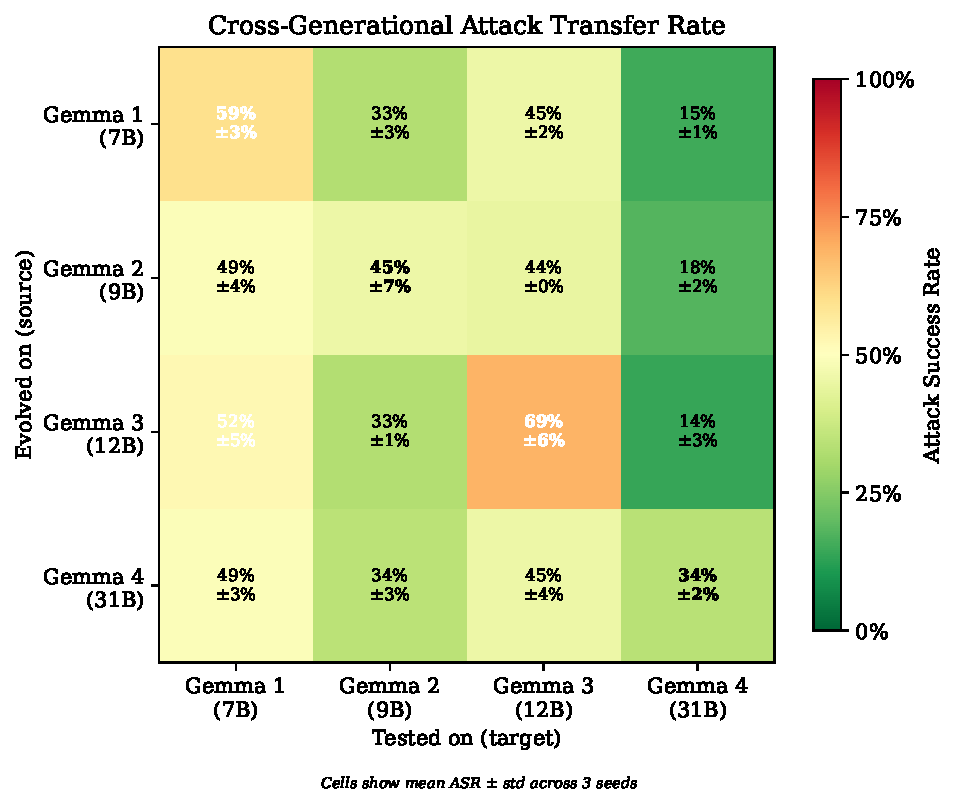
\includegraphics[width=0.6\textwidth]{transfer_heatmap.pdf}
\caption{Cross-generational attack transfer matrix (mean $\pm$ std
across 3 seeds). Cell $(i,j)$ shows the fraction of attacks evolved
against Gemma~$i$ that succeed on Gemma~$j$. Diagonal entries (bold)
are self-evaluation rates.}
\label{fig:transfer}
\end{figure}

\paragraph{Gemma~3 is the easiest transfer target.} Archives from
other generations transfer to Gemma~3 at 44--46\%
($45.5\%$/$44.5\%$/$45.5\%$ from Gemma~1/2/4). A niche decomposition finds Jaccard similarity of 0.66--0.75 among
the successful niches across source archives, indicating substantial
overlap in which (strategy $\times$ encoding $\times$ category) cells
succeed regardless of source.

\paragraph{Gemma~4 resists transfer.} Transfer rates to Gemma~4 are
14--18\% from all sources. Despite Gemma~3's high self-ASR ($68.7\%$),
its attacks do not generalize to Gemma~4, suggesting Gemma~4's
improvements generalize beyond the specific attack distributions
evolved against earlier generations.

\paragraph{Backward transfer is substantial.} Attacks from all
generations transfer to Gemma~1 at $\sim$49--52\%, indicating that
newer probes discover longstanding vulnerabilities.

\subsection{Robustness Across Generations}
\label{sec:results:scaling}

\begin{figure}[t]
\centering
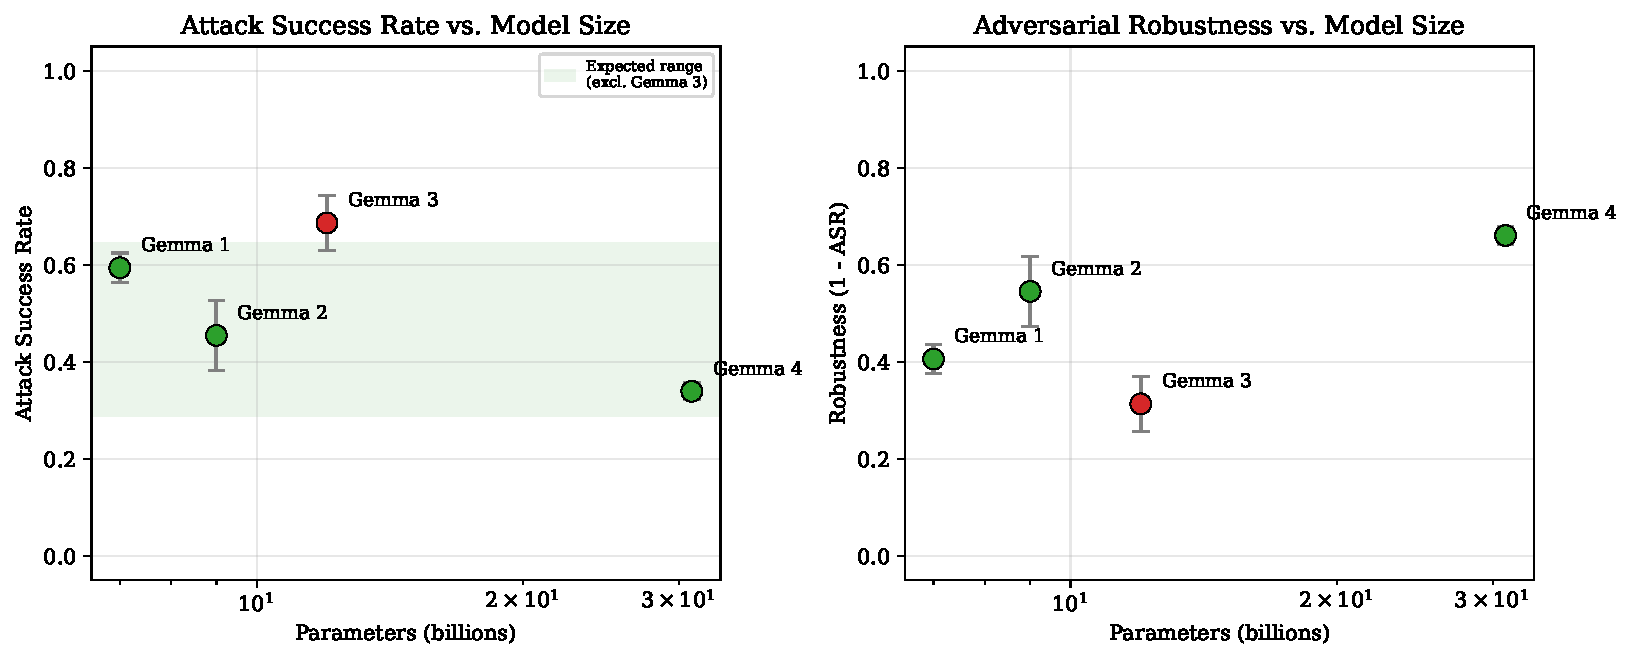
\includegraphics[width=0.95\textwidth]{scaling_curve.pdf}
\caption{Attack success rate (left) and adversarial robustness (right)
vs.\ model size with error bars ($\pm$ 1 std, 3 seeds). The green
shaded region shows the range spanned by Gemma~1, 2, and 4; Gemma~3
(red) falls well outside this range, demonstrating the non-monotonic
pattern. No scaling law is fit; four data points are insufficient.}
\label{fig:scaling}
\end{figure}

Figure~\ref{fig:scaling} plots ASR and robustness ($1 - \text{ASR}$)
against parameter count with error bars. We do not fit a scaling law
to four data points. Instead, we observe that three of the four
models (Gemma~1, 2, 4) are consistent with a gradual improvement
trajectory, while Gemma~3 represents a clear outlier. This
non-monotonic pattern coincides with the architectural transition
from text-only (Gemma~1, 2) to multimodal (Gemma~3, 4), though
Gemma~4's recovery shows that the regression is not an inherent
consequence of multimodal design. Gemma~4's low overall ASR is
driven primarily by near-zero ASR in three categories (chem/bio,
harmful, illegal); misinformation ($76.9\%$) and cybercrime
($48.1\%$) remain high.

\subsection{Vulnerability Fingerprints}
\label{sec:results:fingerprint}

\begin{figure}[t]
\centering
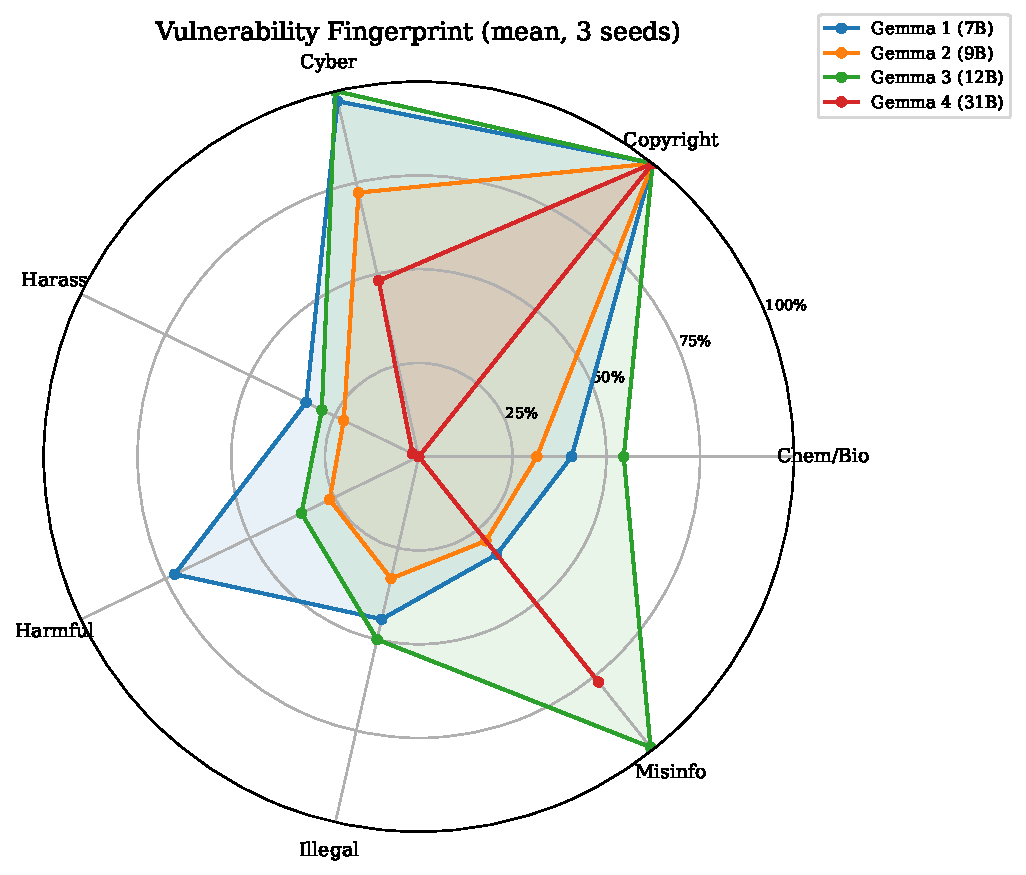
\includegraphics[width=0.55\textwidth]{vulnerability_radar.pdf}
\caption{Vulnerability fingerprints across Gemma generations (mean
ASR per category, 3 seeds). Gemma~2 and Gemma~4 show compact
profiles; Gemma~3's profile is dramatically expanded in
cybercrime and misinformation.}
\label{fig:radar}
\end{figure}

Figure~\ref{fig:radar} presents vulnerability fingerprints as radar
charts. Each model exhibits a distinct profile:
\begin{itemize}
    \item \textbf{Gemma~1}: moderate vulnerability with peaks in
          cybercrime ($97.2\%$) and copyright ($100\%$).
    \item \textbf{Gemma~2}: the most compact profile overall,
          though copyright remains at 100\% and cybercrime at $72.2\%$.
    \item \textbf{Gemma~3}: dramatically expanded in misinformation
          ($99.1\%$) and cybercrime ($100\%$). Only harassment
          shows continued improvement.
    \item \textbf{Gemma~4}: achieves 0\% ASR in chem/bio, harmful,
          and illegal, but copyright ($100\%$) and misinformation
          ($76.9\%$) remain elevated.
\end{itemize}

%% ============================================================================
\section{Discussion}
\label{sec:discussion}

\paragraph{Safety regression in Gemma~3.}
The most surprising finding is Gemma~3's safety regression, which is
statistically significant versus Gemma~2 ($p = 0.030$, paired bootstrap
across 3 seeds). We hypothesize this is related to the introduction of
multimodal capabilities: Gemma~3 was the first Gemma generation with
vision-language support (architecture: \texttt{Gemma3ForConditionalGeneration}),
requiring substantial architectural changes that may have disrupted
safety-trained text representations. The fact that harassment, the
category most explicitly targeted by safety training across all
LLMs, shows a broadly declining trajectory even through Gemma~3
($33.3\% \to 22.2\% \to 28.7\% \to 1.9\%$) supports this
interpretation: category-specific safety training was maintained,
but general robustness was compromised.
Alternative hypotheses that the data does not rule out include
(a)~idiosyncratic training-data-mix issues specific to Gemma~3
unrelated to modality, (b)~changes in the RLHF/DPO recipe between
generations, and (c)~increased model capability raising the ceiling
on evolutionary search. Distinguishing these would require access to
training details, which we do not have.

\paragraph{Gemma~4's recovery.}
Gemma~4 achieved the lowest overall ASR in the family
($33.9\% \pm 1.8\%$) despite being multimodal, suggesting that the
safety regression in Gemma~3 was addressable. The extremely low
transfer rate from Gemma~3 to Gemma~4 ($14.0\% \pm 2.7\%$) indicates
that Gemma~4's improvements generalize beyond the specific attack
distributions evolved against Gemma~3. However, Gemma~4's safety is
category-heterogeneous: three categories reach 0\% ASR while
misinformation ($76.9\%$) and cybercrime ($48.1\%$) remain high.

\paragraph{Judge sensitivity and copyright.}
Copyright-category ASR is consistently highest across all generations
under our 8B judge. However, a second-judge audit using
Llama-3.1-70B-Instruct ($N = 52$ samples with stored responses) found
that the 70B judge classified only 50\% of copyright responses as
harmful (vs.\ 100\% for the 8B judge), suggesting that the 8B
judge's harm threshold for copyright is more permissive. Overall,
the two judges agree on refusal (96.2\%) but show weak agreement on
harm classification ($\kappa = 0.15$). The second-judge audit covered
52 samples, which limits per-category resolution; a larger audit would
be needed to characterize judge disagreement per category. Per-category
ASRs should be interpreted with this caveat.

\paragraph{What we claim and what we do not.}
With four data points we cannot distinguish a U-shaped curve from
noise. What we \emph{can} say is that the Gemma~2 $\to$ Gemma~3
regression is statistically significant and large ($+23.2$ percentage
points), and that the transfer matrix provides converging evidence
(Gemma~3 is the easiest transfer target from all directions).

\paragraph{Implications for safety evaluation.}
Static benchmarks would miss the non-monotonic trajectory entirely.
Architectural changes (such as adding multimodal capabilities) should
trigger comprehensive safety re-evaluation. The distinction between
Gemma~3 (high self-ASR, high inbound transfer) and Gemma~4 (low
self-ASR, low inbound transfer) is only visible through
cross-generational transfer analysis.

\paragraph{Limitations.}
\begin{itemize}
    \item Three seeds per model provide reproducibility estimates but
          limited statistical power. The Gemma~3 $\to$ Gemma~4
          improvement, while large ($-34.8$ pp), does not reach
          $p < 0.05$. Additional seeds would tighten confidence
          intervals.
    \item Single model family (Gemma) for generational analysis;
          findings may not generalize to other families.
    \item The 8B judge shows weak agreement ($\kappa = 0.15$) with a
          70B judge on harm classification, particularly for
          copyright. Per-category ASRs are judge-dependent.
    \item HarmBench coverage: 400 behaviors across 7 categories is
          comprehensive but not exhaustive.
    \item Evolutionary probe explores a subset of the attack space;
          absence of a successful attack does not prove safety.
    \item We study only the text modality; Gemma~3 and 4's vision
          capabilities may present additional attack surfaces not
          captured here.
\end{itemize}

%% ============================================================================
\section{Conclusion}
\label{sec:conclusion}

We have presented a methodology for longitudinal safety evaluation of LLMs
using quality-diversity evolution as a differential probe. Applied to four
generations of Google's Gemma models with 3 independent seeds per model,
we find that:

\begin{enumerate}
    \item Safety alignment does not improve monotonically across model
          generations. Gemma~3 represents a statistically significant
          regression ($68.7\% \pm 5.7\%$ ASR vs.\ Gemma~2's
          $45.5\% \pm 7.2\%$; $p = 0.030$).
    \item Cross-generational attack transfer is generation-dependent:
          attacks from other generations transfer to Gemma~3 at
          $\sim$45\% but only 14--18\% to Gemma~4, suggesting
          Gemma~4's improvements generalize across attack
          distributions evolved against earlier generations.
    \item Vulnerability profiles are category-dependent:
          copyright-category ASR is consistently highest across all
          generations under our 8B judge (though this specific number
          is sensitive to judge choice), Gemma~4 achieves 0\% in
          three categories, but misinformation remains elevated
          ($76.9\%$) even in the safest generation.
\end{enumerate}

These results underscore the need for \emph{adaptive, longitudinal}
safety evaluation. Static benchmarks provide a snapshot; evolutionary
probing with transfer analysis reveals the \emph{trajectory} of safety
alignment. We advocate for model developers to publish generational
safety analyses alongside capability benchmarks, and for the research
community to develop standardized protocols for cross-version
safety comparison.

%% ============================================================================

\begin{ack}
Compute for Gemma experiments was provided by RunPod (NVIDIA H200
and RTX~4090 instances).
\end{ack}

\bibliographystyle{plainnat}
\bibliography{references}

\end{document}
